\documentclass[DM,authoryear,toc]{lsstdoc}
% lsstdoc documentation: https://lsst-texmf.lsst.io/lsstdoc.html
\input{meta}

% Package imports go here.

% Local commands go here.

%If you want glossaries
%\input{aglossary.tex}
%\makeglossaries

\title{Campaign Tooling -- tools for generating, monitoring and tracking data processing campaigns}

% Optional subtitle
% \setDocSubtitle{A subtitle}

\author{%
Brian Yanny, Colin Slater, Sergey Padolski, Yusra AlSayyad, Hsin-Fang Chiang, Huan Lin
}

\setDocRef{RTN-023}
\setDocUpstreamLocation{\url{https://github.com/lsst/rtn-023}}

\date{\vcsDate}

% Optional: name of the document's curator
% \setDocCurator{The Curator of this Document}

\setDocAbstract{%
Tools for working with the Butler to query for status of data collections to generate processing campaigns, for working with BPS, PanDA,  Condor or other workflow systems to monitor campaigns; tools to track success and failure of campaigns, past and present. Requirements described.
}

% Change history defined here.
% Order: oldest first.
% Fields: VERSION, DATE, DESCRIPTION, OWNER NAME.
% See LPM-51 for version number policy.
\setDocChangeRecord{%
  \addtohist{1}{YYYY-MM-DD}{Unreleased.}{Brian Yanny}
}


\begin{document}

% Create the title page.
\maketitle
% Frequently for a technote we do not want a title page  uncomment this to remove the title page and changelog.
% use \mkshorttitle to remove the extra pages

% ADD CONTENT HERE
% You can also use the \input command to include several content files.

\section{Introduction and Definitions}

Data Processing for Rubin occurs at several levels,
as described in https://dmtn-137.lsst.io. 

A campaign is a set of pipelines run in quantum-graph prescribed order and
parallelism on a input collection producing an output collection.

Some examples of campaigns might be:

1. Generate a set of flat fields by combining a collection of input raw flats,
grouped by filter and detector.  The input collection may be all raw flat
exposures obtained last night or over the last 10 nights, with 'defective'
raw flats removed from the collection 'in advance'.

2.  Process last night's visits through instrument-signature-removal, source 
detection and measurement resulting in corrected images and catalogs
for each exposure/detector combination.

3. Generate a photometric calibration solution (FGCM) over a large area
of sky using catalogs of detected objects for a set of exposure/detectors.

4. Combine all corrected detector images that overlap a specific patch
on the sky to using a specific photometric and using (or generating) an 
astrometric calibration into a coadd image.

Each campaign can be specified by specifying a set of inputs, pipelines,
software stack versions, and outputs.

The quantum graph for a campaign understands what steps depend on which
previous steps and when a step may be in parallel over a large set of
individual inputs.

A set of campaigns may run the same (or similar) graph or steps over 
different input collections.

Campaigns are driven by yaml-style configuation scripts which are launched
by a command such as 'bps submit'.

It would be useful, when managing large sets of campaigns, such as for
nightly or annual Data Release Processing DRP or for Prompt/Alert systems, 
to track all campaigns submitted as well as their status with links to
logs of individual jobs (tasks) within the campaigns.  System performance
metrics on campaigns may also find it useful to connect directly with
a campaign tracking system.

The purpose of this document is to describe requirements on such a campaign
tracking and monitoring system.

https://rtn-013.lsst.io


\begin{figure}
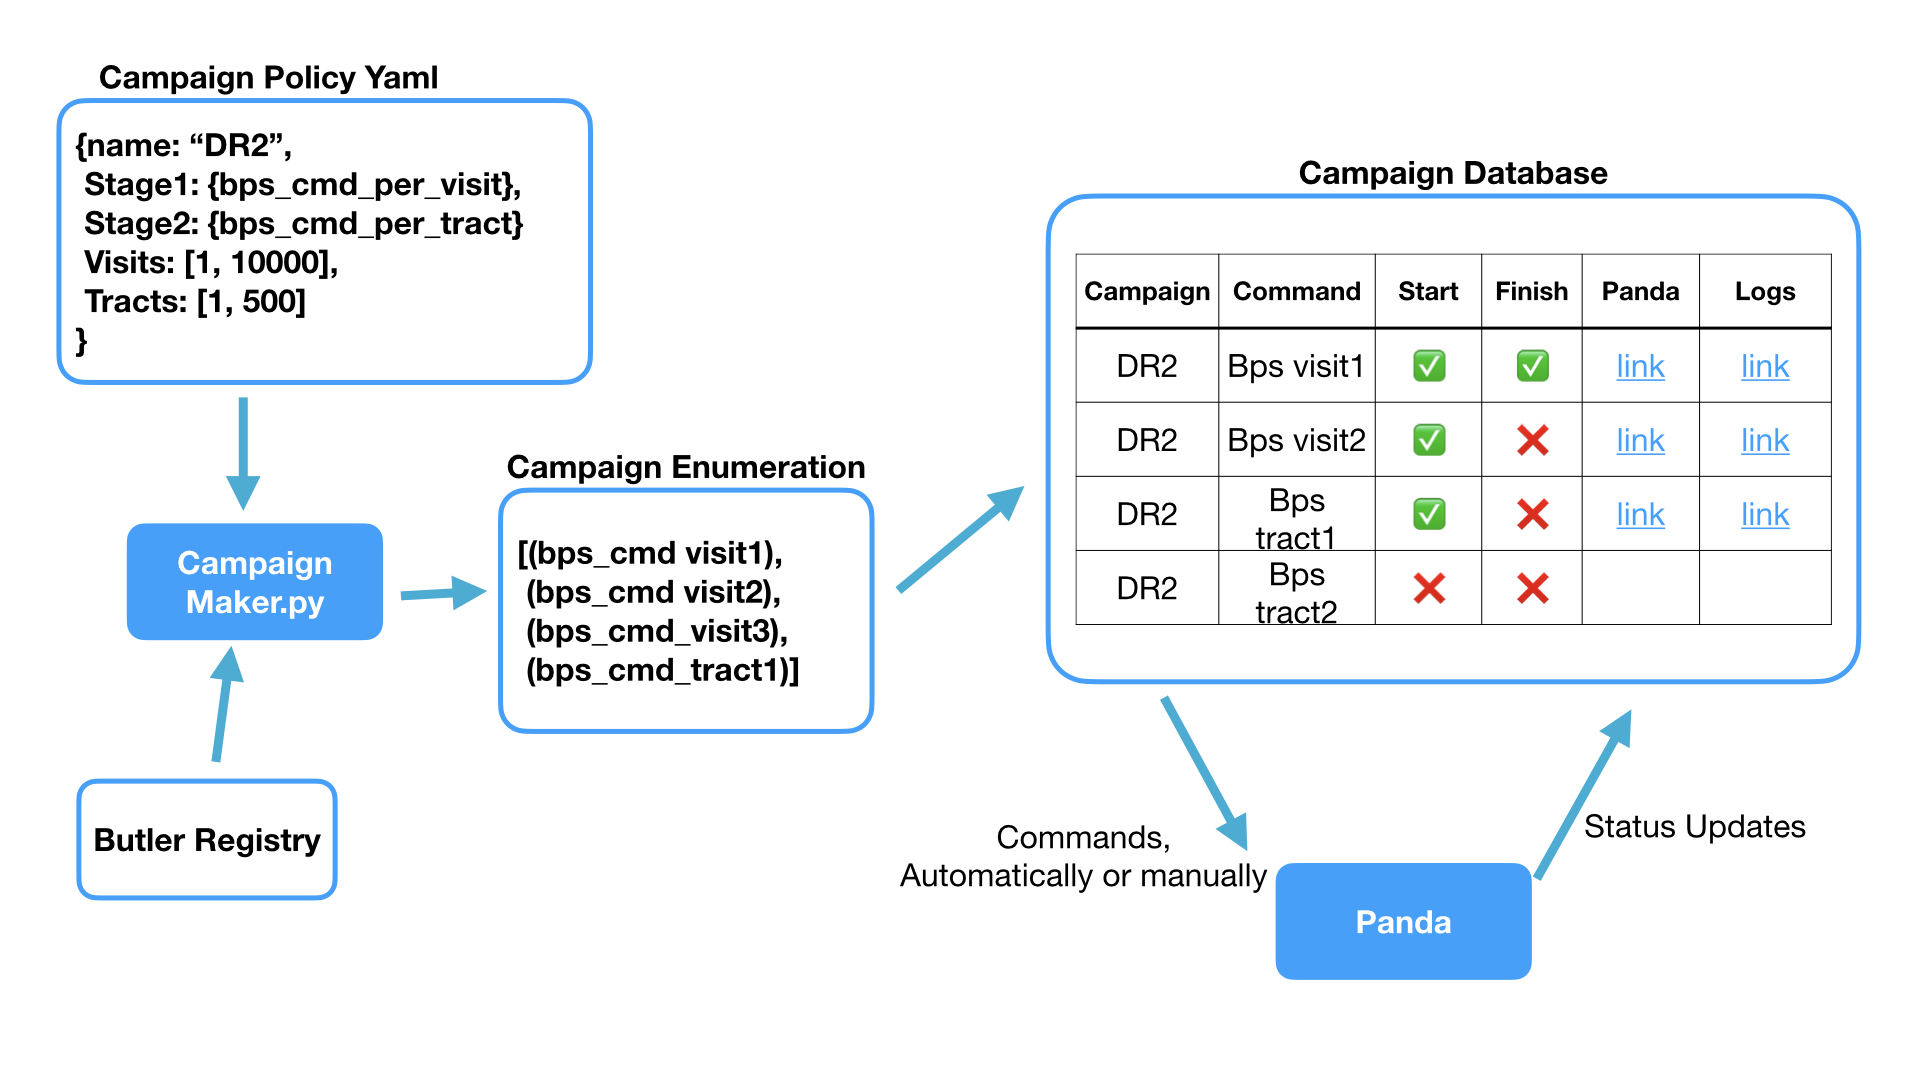
\includegraphics[width=\textwidth]{CampaignTooling.jpg}]
\caption{Diagram of Campaign generation (left) and monitoring system (right).
Credit: C. Slater}
\end{figure}

\begin{figure}
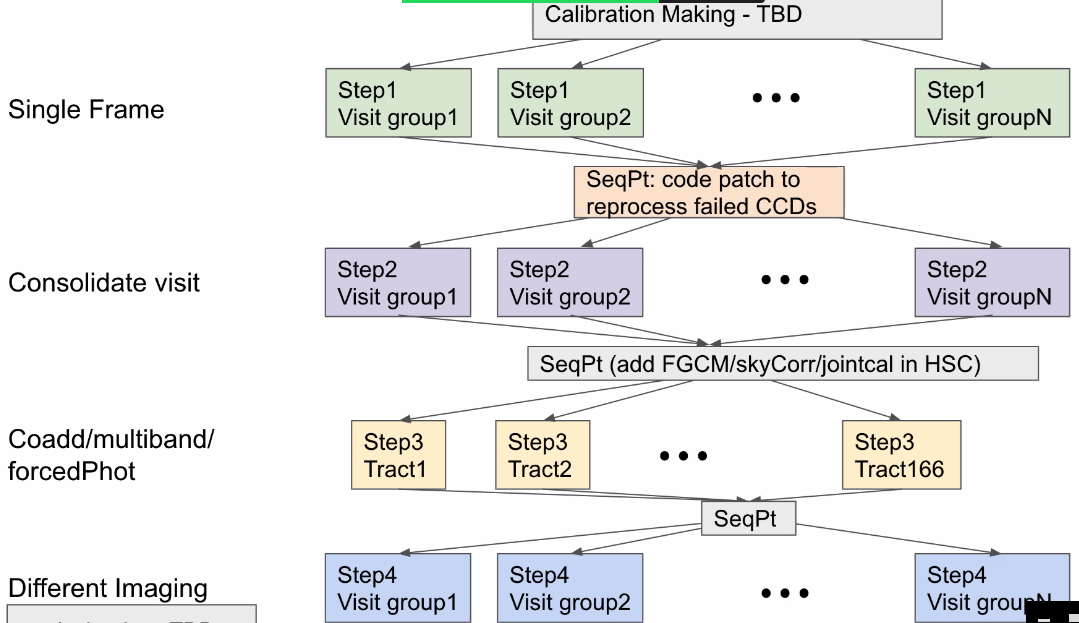
\includegraphics[width=\textwidth]{analdrp.png}]
\caption{Diagram of Data Release Processing data flow.
Credit: Y. AlSayyad, H. Chiang}
\end{figure}


\section{Campaign Generation and Tracking Requirements}

 To generate processing campaigns and track them these features are desired:

	\begin{enumerate}

	\item Ability to access up-to-date source of inputs to-be-processed
		into outputs and their current state 
		(already processed, processed and flagged bad, 
		in processing)

	\begin{itemize}
	
	\item May wish to avoid constantly hitting the butler for
	its contents -- so may wish to have another active source
	of inputs and status of processing -- i.e. another database
	which would only occasionally check with the butler to sync up


	\end{itemize}

	\item Ability to generate BPS submit yaml configs 
	(or other top level workflow submit scripts) which request processing
	of subset of inputs needing to be processed, pipelines to be run,
	outputs described.  This could, for instance, be achieved by having
	a set of template yaml configs -- one for each procesing step
	(Single Frame, Consolidate Visit, Photo calib FGCM, 
	astrometric calib skyMap, Coadd/forced Photometry, Difference
	Imaging Analysis) where a 'sed' script or similiar would fill in
	a visit list, a src catalog list, a tract list, etc

	\begin{itemize}

	\item Should be able to 'split' a large set of inputs into
	serveral managable sized pieces.  For instance, DP0.2 consists of
	about 40,000 visits, and a typical Rubin night of observing will
	take 1,000-2,000 science exposures.   So a managable unit for
	single visit processing might be of size 1000 exposures/visits and
	a DP0.2 processing would split the 40,000 visits into 1000 visit
	groups.  Consideration should be given to how long (wallclock time)
	a single campaign 'unit' may be run and to not generally exceed 
	24 hours to a few days to avoid interruptions from downtimes.
	Also depends on ability of system to recover from interruptions and
	continue without needing to restart the whole campaign from
	the beginning.
	

	\item  Should allow(?) 'last minute editing' of configs before
	submission to tweak something, change a pipeline version or
	visit input list

	\item each campaign should be identified by some unique id string, 
	perhaps same as workflow manager identifying string?

	\end{itemize}

	\item Ability to store and manage a set of BPS submit scripts 
	(or equivalent).
	For instance, as each BPS submit yaml is performed, the yaml
	script contents could be saved in a database with metadata such
	as time of submission, location of physical processing
	(SLAC, IN2P3, UK, Cloud, user-laptop), current state (non started,
	running, finished-no-errors, finished-with-errors)


	\item Ability to quickly access and view logs of each 
	campaign's individual tasks/jobs to determine errors

	\item Ability to view overall state of running and recently
	completed campaigns, without being overwhelmed by long-ago completed
	or abandoned campaigns.

	\item Ability to straight-forwardly dump dataids (or filenames
	with paths) and metadata (exposureid, filter) of inputs or outputs
	from some specific job or task of the processing campaign to
	track down issues and errors.  This ability may be present already
	but some 'helper' scripts could simplify the process.

	\item Ability to watch, in realtime, as jobs or tasks within
	a campaign or set of campaigns are running.  There is a tool	
	called 'BPS report' which does this at some level, showing how
	many individual inputs in a campaign set have been processed
	so far.

	\end {enumerate}

\appendix
% Include all the relevant bib files.
% https://lsst-texmf.lsst.io/lsstdoc.html#bibliographies
\section{References} \label{sec:bib}
\renewcommand{\refname}{} % Suppress default Bibliography section
\bibliography{local,lsst,lsst-dm,refs_ads,refs,books}

% Make sure lsst-texmf/bin/generateAcronyms.py is in your path
\section{Acronyms} \label{sec:acronyms}
\addtocounter{table}{-1}
\begin{longtable}{p{0.145\textwidth}p{0.8\textwidth}}\hline
\textbf{Acronym} & \textbf{Description}  \\\hline

BPS & Batch Production Service \\\hline
DC2 & Data Challenge 2 (DESC) \\\hline
DESC & Dark Energy Science Collaboration \\\hline
DF & Data Facility \\\hline
DM & Data Management \\\hline
DMTN & DM Technical Note \\\hline
DMTR & DM Test Report \\\hline
DP0 & Data Preview 0 \\\hline
DR1 & Data Release 1 \\\hline
DRP & Data Release Production \\\hline
FGCM & Forward Global Calibration Model \\\hline
FTS & File Transfer Service \\\hline
HSC & Hyper Suprime-Cam \\\hline
IDF & Interim Data Facility \\\hline
IN2P3 & Institut National de Physique Nucléaire et de Physique des Particules \\\hline
IP & Internet Protocol \\\hline
LDM & LSST Data Management (Document Handle) \\\hline
LSST & Legacy Survey of Space and Time (formerly Large Synoptic Survey Telescope) \\\hline
PanDA &  Production ANd Distributed Analysis system \\\hline
RTN & Rubin Technical Note \\\hline
SLAC & SLAC National Accelerator Laboratory \\\hline
SQL & Structured Query Language \\\hline
SST & Subsystem Science Team \\\hline
UK & United Kingdom \\\hline
URL & Universal Resource Locator \\\hline
US & United States \\\hline
bps & bit(s) per second \\\hline
stdout & standard output \\\hline
\end{longtable}

% If you want glossary uncomment below -- comment out the two lines above
%\printglossaries





\end{document}
